\section{Results}
\label{sec:chap_slam_results}

In this section, we evaluate the performance of the place recognition algorithm on our three datasets. We then compare the results between the unstructured and structured environments as well as between the SICK and the Velodyne acquisitions. 

\subsection{Performance Evaluation}
\label{ssec:chap_slam_performance_evaluation}

In order to evaluate the place recognition performance, two elements are required. Firstly, a rule for labeling two positions of the real world as belonging (or not) to the same place, and secondly, the algorithm prediction for two input scans. In the following subsection, we will first discuss these two elements and present the resulting data. Afterwards, we will conduct the performance evaluation itself.


\subsubsection{Real World Places}
The notion of a place can be variable, but the closer two points of the space are to each other, the more likely they are to be considered in the same place. Therefore, we use the real world physical distance between two acquisitions as an indicator of the likelihood that they represent the same place. We will now discuss the method used to determine the distance between scans. 

We first used the robot odometry as a rough approximation of the relative pose between two subsequent scans. In order to reduce the pose estimation error, we then used the \gls*{icp} algorithm to align the two point clouds and adjust the odometry accordingly. These steps were performed sequentially for all scans of the first loop. This technique can not be independently repeated for the second loop, because the difference in error accumulation would cause a discrepancy between the resulting path of the two loops. To address this problem, the \gls*{icp} odometry adjustment of the second loop was performed relative to the first loop. To do this, we first align the first scan of the second loop relative to the first scan of the first loop using \gls*{icp}. Thereafter, each scan of the second loop was adjusted with respect to the scan of the first loop theoretically being closest, considering the last corrected pose and the movement of the robot. Figure~\ref{fig:chap_slam_results_paths} illustrates the resulting paths, as well as the position of each scans for our three datasets. Note that this is a \gls*{2d} representation for which the vertical component was ignored. This figure shows the absence of discrepancy between the two loops of each dataset.

With the corrected odometry it is possible to easily obtain the distance between two scans. To do this, one can simply calculate the norm of the difference in position between the two scans. On the other hand, given the accumulated odometry error, the relative position between the last scan of a loop $L_i$ and the first scan of a loop $L_j$ (including $i=j$) can be significant. The relative error generally also increases over time (with each move to a new acquisition). To reduce the impact of these problems, we used \gls*{icp} to determine the relative pose for all pair \textit{($L_i$ first scan, $L_j$ last scan)}. With these relative poses, it was possible to create the reverse sequential path between two scans. Finally, we use the path for which the scans are closest in terms of acquisition numbers (sequential or reverse) for the final calculation of the distance.

Note that all alignments have been visually inspected to ensure that \gls*{icp} had indeed converged to a valid solution. When this was not the case, the odometry provided by the robot was manually adjusted to enable this convergence. The second line of Figure~\ref{fig:chap_slam_results} show the resulting distances matrices for all pair of scans of each of our three datasets. Note that a distance function is by definition symmetrical, therefore producing a symmetrical matrix. The values on the main diagonal represent the distance between a scan and itself and are therefore null. A secondary diagonal of low values is produced by the small distances between the scans of the first and the second loop. Finally, because we tried to stop the loop acquisitions approximately at the starting point, we observe small values at those junction points (at the bottom left corner for instance).

\begin{figure}[H]
    \centering
    \subfloat[]{\label{fig:building_paths_plot}}{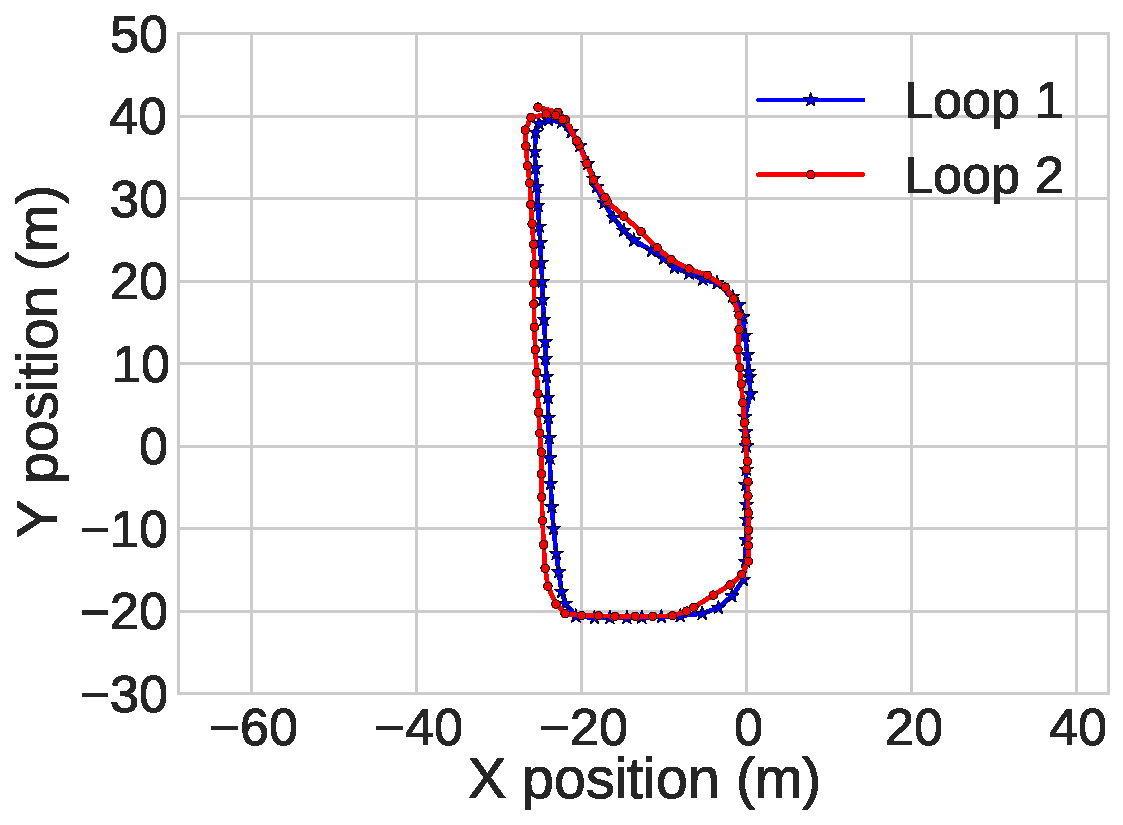
\includegraphics[width=0.6\linewidth]{img/chap_slam/building_paths.pdf}}
    \subfloat[]{\label{fig:forest_paths_plot}}{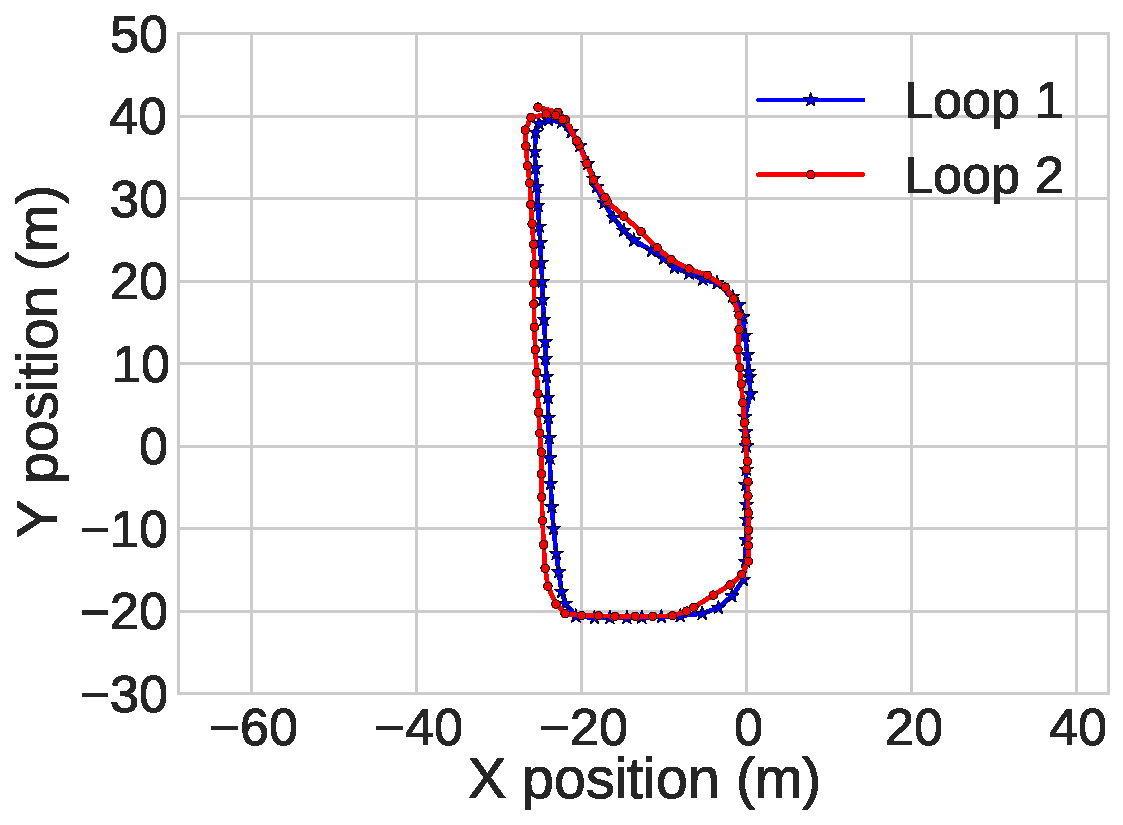
\includegraphics[width=0.6\linewidth]{img/chap_slam/building_paths.pdf}}
    \subfloat[]{\label{fig:velodyne_paths_plot}}{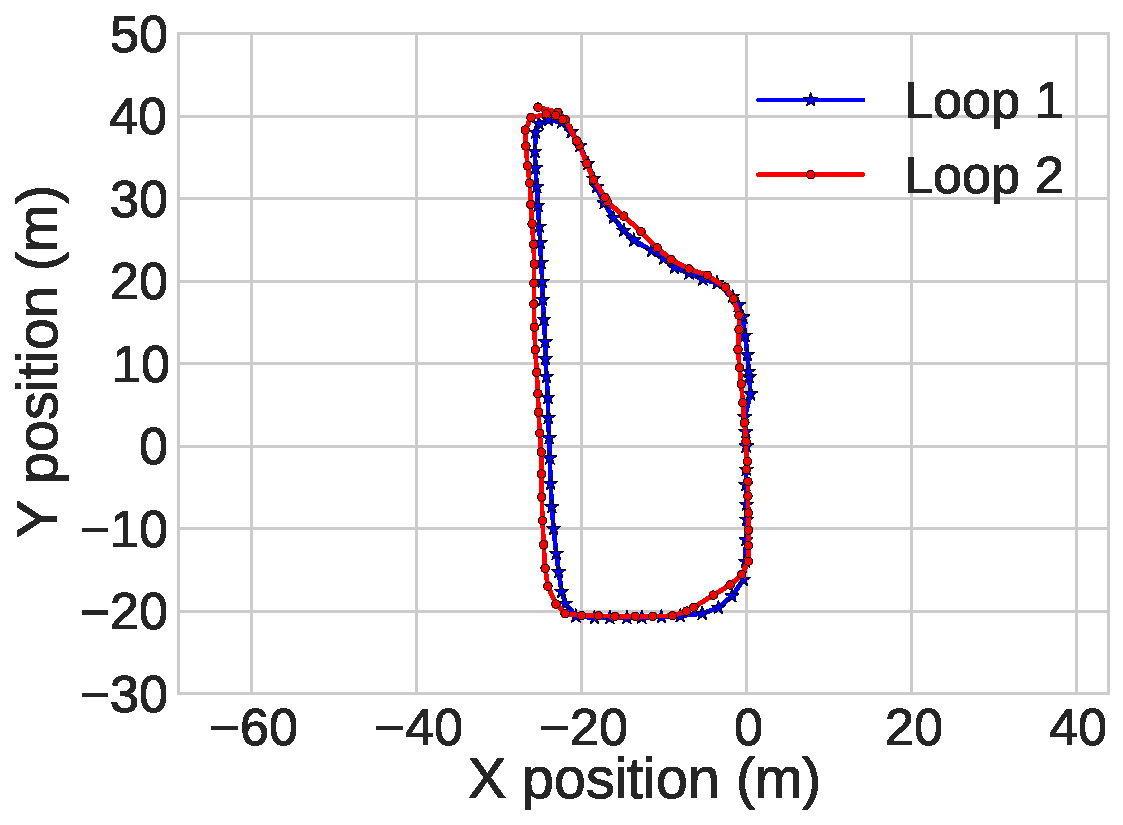
\includegraphics[width=0.6\linewidth]{img/chap_slam/building_paths.pdf}}
    \caption[todo]{\todo{Hum... too big?...}}
    \label{fig:chap_slam_results_paths}
\end{figure}


\subsubsection{Algorithm Prediction}
For our experiments, we used a \textit{C++} implementation of the place recognition algorithm developed by Bastian Steder, who provided us the source code. The software, resulting from the compilation of this code, allowed us to obtain a score between 0~and~1 for each pair of scan in the database. As explained in Section~\ref{sec:chap_slam_algo}, this score reflects the system belief that the two scans represents the same place. More precisely, when the score is zero, the algorithm believes there is no chance that the scans originate from the same place, and when the score is one, the algorithm is certain that they do not originate from the same place.

The second row of Figure~\ref{fig:chap_slam_results} represents the scores matrices for our three datasets. Note that the main diagonal of these matrices is the score of a scan compared to itself, which always results in a value of~1. It is possible to observe a slight asymmetry in the matrices caused by the non-symmetric function used for calculating scores. Note that, for our results analysis, we will only consider the values from the area below the main diagonal.


\subsubsection{Evaluation}
\label{ssec:chap_slam_results_evaluation}

Considering the two previous subsections, we should expect to see a high score for a pair of close scans and a low score for a pair of remote scans. This relationship can actually be observed by comparing the distances matrices and the scores matrices (first and second rows of Figure~\ref{fig:chap_slam_results}). The third row of Figure~\ref{fig:chap_slam_results} also illustrates this relation by a scatter plot, where each pair of scans is represented by a data point based on the distance between the scans and the score produced by the place recognition algorithm. In addition to observing the expected correlation from these figures, it shows no outliers.

While it is interesting to observe a continuous relationship between these values, practical uses of place recognition generally require a binary labeling of each pair of scans (either originating from the same place or not). To determine the ground truth labels (real world places), a threshold will be defined on the distance between the scans. All pairs of scans closer than this distance threshold will be considered as being in the same place. Regarding the algorithm prediction labels, a threshold will be set on the output score. All pair of scans obtaining a score higher than this threshold will be labeled as originating from the same place. Table~\ref{tab:chap_slam_results_labeling} summarises how these thresholds will be used to label data and analyse results.

As indicated in the introduction of this chapter (Section~\ref{sec:chap_slam_intro}), \gls*{slam} algorithms generally use place recognition to detect loop closures. If two scans are identified as coming from the same place, but this is not the case (i.e. a false positive), the \gls*{slam} algorithm will create a link that should not exist in the map. When doing \gls*{slam}, creating such a link is more damaging than ignoring a genuine link. For this reason, the place recognition algorithm used should be set to avoid getting false positives. In our case, we can respect this constraint by choosing the threshold on the score based on the distance threshold. This is represented by the line of the plots of the third row in Figure~\ref{fig:chap_slam_results}.

\todo{Here I am... How should I present de recall rate / precision...}

\begin{table}[H]
    \centering
    \begin{tabular}{@{}l|ll@{}}
        \toprule
                                  & \textbf{$D < T_{distance}$} & \textbf{$D >= T_{distance}$} \\
        \hline
        \textbf{$S > T_{score}$}  & True Positive (TP)          & False Positive (FP) \\
        \textbf{$S <= T_{score}$} & False Negative (FN)         & True Negative (TN) \\
        \bottomrule
    \end{tabular}
    \caption[Summary of scans pairs labeling for results analysis]{A summary of scans pairs labeling for results analysis. $D$ represents the distance between the two scans, $S$ represents the place recognition algorithm output score. $T_{distance}$ and $T_{score}$ represent the thresholds for the distance and the score, respectively.}
    \label{tab:chap_slam_results_labeling}
\end{table}


\subsection{Comparative Analysis}
\label{ssec:chap_slam_comparative_analysis}

\subsection{Structured and Unstructured Environments}
\label{ssec:chap_slam_struct_vs_forest}
\begin{itemize}
    \item Because distance is smaller on avg in the forest, cause parallax
    \item Also more occlusion, but this also why the env. is complex. As said earlier range img kind of deal with it.
\end{itemize}

\subsection{SICK and Velodyne \gls*{lidar}s}
\label{ssec:chap_slam_sick_vs_velodyne}


\begin{figure}[H]
    \centering
    \subfloat[]{\label{fig:building_scores_matrix}}{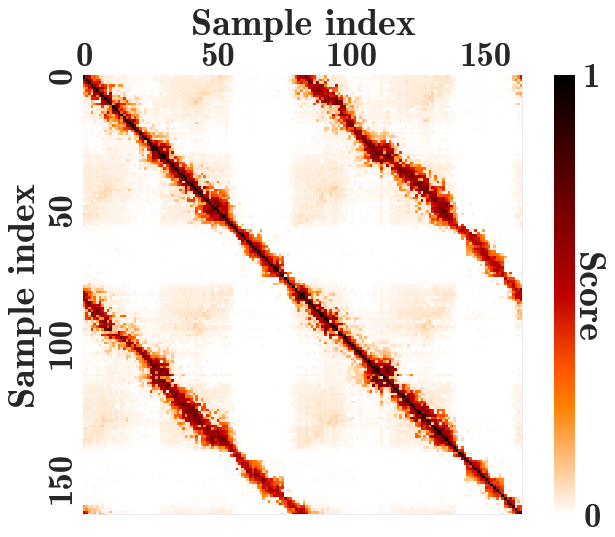
\includegraphics[width=0.31\linewidth]{img/chap_slam/building_scores_matrix.png}}
    \subfloat[]{\label{fig:forest_scores_matrix}}{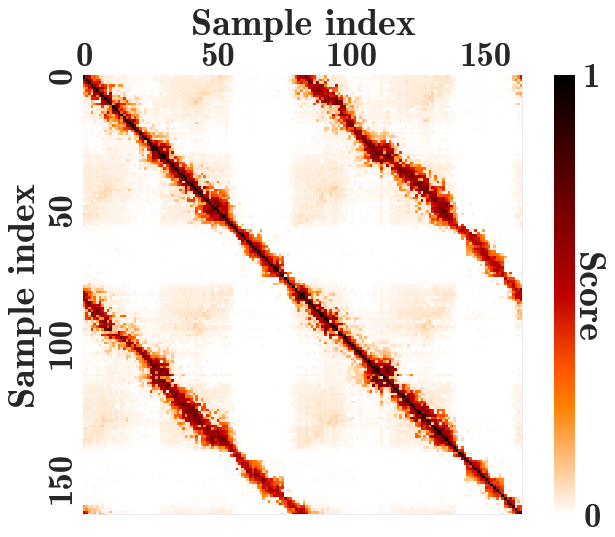
\includegraphics[width=0.31\linewidth]{img/chap_slam/building_scores_matrix.png}}
    \subfloat[]{\label{fig:velodyne_scores_matrix}}{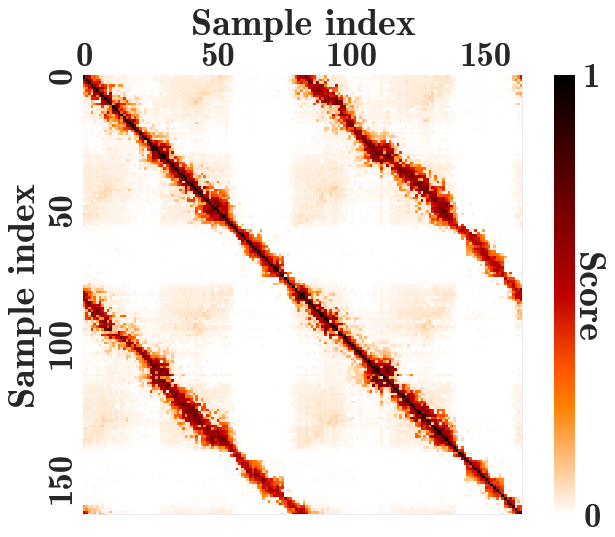
\includegraphics[width=0.31\linewidth]{img/chap_slam/building_scores_matrix.png}} \\

    \subfloat[]{\label{fig:building_distances_matrix}}{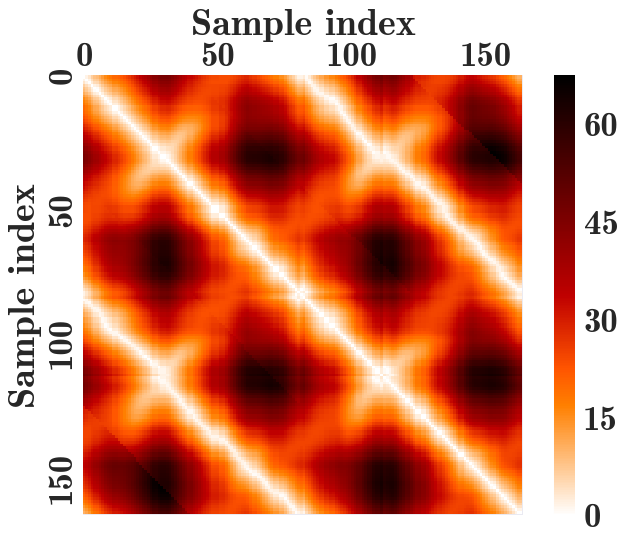
\includegraphics[width=0.31\linewidth]{img/chap_slam/building_distances_matrix.png}}
    \subfloat[]{\label{fig:forest_distances_matrix}}{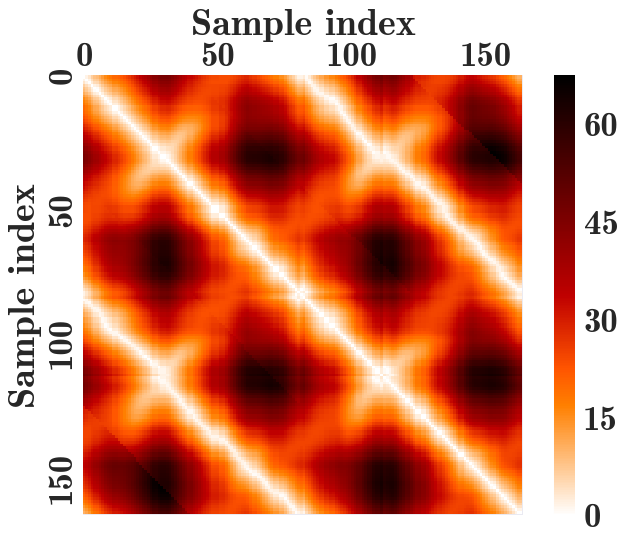
\includegraphics[width=0.31\linewidth]{img/chap_slam/building_distances_matrix.png}}
    \subfloat[]{\label{fig:velodyne_distances_matrix}}{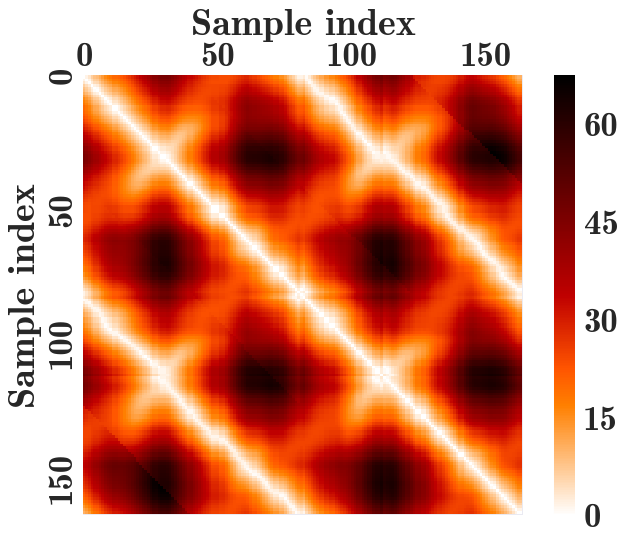
\includegraphics[width=0.31\linewidth]{img/chap_slam/building_distances_matrix.png}} \\

    \subfloat[]{\label{fig:building_distances_scores_plot}}{\includegraphics[width=0.31\linewidth]{img/chap_slam/building_distances_scores_plot.pdf}}
    \subfloat[]{\label{fig:forest_distances_scores_plot}}{\includegraphics[width=0.31\linewidth]{img/chap_slam/building_distances_scores_plot.pdf}}
    \subfloat[]{\label{fig:velodyne_distances_scores_plot}}{\includegraphics[width=0.31\linewidth]{img/chap_slam/building_distances_scores_plot.pdf}}

    \subfloat[]{\label{fig:building_recall_plot}}{\includegraphics[width=0.31\linewidth]{img/chap_slam/building_recall_plot.pdf}}
    \subfloat[]{\label{fig:forest_recall_plot}}{\includegraphics[width=0.31\linewidth]{img/chap_slam/building_recall_plot.pdf}}
    \subfloat[]{\label{fig:velodyne_recall_plot}}{\includegraphics[width=0.31\linewidth]{img/chap_slam/building_recall_plot.pdf}}
    \caption[todo]{\protect\subref{fig:result_matrix_structured} is the confusion matrix for both loops of the structured dataset (XX scans) and \protect\subref{fig:result_curve_structured} is the recall curve. \protect\subref{fig:result_matrix_forest} and \protect\subref{fig:result_curve_forest} are the corresponding matrix and recall curve for the unstructured dataset and \protect\subref{fig:result_matrix_forest} and \protect\subref{fig:result_curve_forest} are for the unstructured dataset using the velodyne.}
    \label{fig:chap_slam_results}
\end{figure}
